\chapter{Core reference}
\section{\module{pyDCPU} --- 
        \textbf{Py}thon \textbf{D}ata \textbf{C}ollect and \textbf{P}rocess \textbf{U}nit}

\declaremodule{}{pyDCPU}       

\moduleauthor{Hannes Matuschek}{hmatuschek@gmx.net}


\modulesynopsis{This is the reference for the core-library of PPLT System.}

The \module{pyDCPU} module provides all needed core methods and functions, to
get a PPLT system running. The library implements the basic features like 
loading modules (Master/Exporter), manageing the symboltree 
(create/move/delete/chmod/chown/chgrp/...) and manageing the user
data base. Basicly the \module{pyDCPU} library provides all the functionality
of the PPLT system. 

\subsection{Concept} 
The core of the PPLT system have to provide all the functionality to access devices
by master-slave based communication channels and handle the values read back into
a central place. Also these values should be served to other applications, indipendent
from the interface the application use. So the core is splitted into three major parts.

\begin{figure}[ht]
    \centering
    \label{cDCPU}
    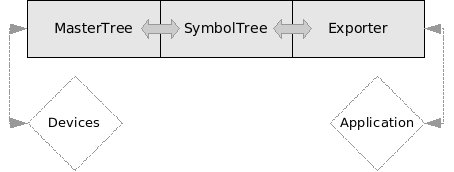
\includegraphics[scale=1]{cDCPU.png}
    \caption{Parts of the core.}
\end{figure}

The first called \textit{MasterTree}. This provide the access to the devices. The 
second part called \textit{SymbolTree} holds all values in a filesystem like 
hierachie. The last part, the \textit{Exporters}, serves the symboltree to other
applications like a visualisation. This concept is very common for this kind of 
problems. 

\subsubsection{The MasterTree}
To access the devices a master-slave based communication is often used. This are 
for example the common BUSes and also TCP/IP like networks. All these protocols
have one basic concept; they are seperable into layers. Each layer encapsulate 
an element of the communication.  For TCP/IP this is the famouse OSI reference 
model. So it is usefull to implement each layer of the communication channel
into separate modules to have the facility to reuse some of the modules. By
this you only need to implement these layers of the communication, that aren't
implemented yet to access a new device. For example if you want to access
a unsupported device that uses an allready implemented BUS you'll need only
to write a module that implements the command messages for this device.

A common way to seperate the communication is to differ between the used
interface, transport-protocol, and command-messages. The interface provides
the access to the BUS wardware, for example the serial-interface. The 
transport-protocol or BUS protocol uses the interface and generate valid 
messages that reaches the device. The module that generates the 
command-messages uses the transport-protocol to send the messages to the
device and to wait for an answer.  

\begin{figure}[ht]
    \centering
    \label{fig:cMasterTree}
    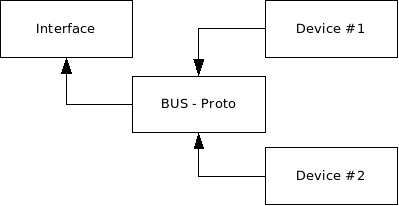
\includegraphics[scale=1]{cMasterTree.png}
    \caption{Scheme of MasterTree concept with shared interface and BUS modules.}
\end{figure}

An common cenario would be: You want to get a value from a device. So
you read from the module-object that implements the command messages.
This module will send a command-message over the BUS (protocol and interface)
to the device. Then the module will waits for an answer of the device
by reading from the BUS (over protocol and interface module). The
answer will be dispatched and you'll get the value.

If one module read from or writes to an other module the modules
will be locked and no other module can access these modules. By this way 
BUS collisions are avoided. And on the other hand if you want to access
two devices that are connected to the same BUS, you'll setup a 
MasterTree where the device-modules \#1 and \#2 share the modules for the 
interface and BUS. Now you see why the MasterTree is called a tree (forest 
would be better). The root of each tree is the interface and the leafes are 
the devices.

To get the all module work together a clear API between the modules have
to be defined, so that you don't have to adjust the modules to work together
with other/new modules. 

\subsubsection{The SymbolTree}
Once the access to the devices is seted up, you need to care about what values 
should be served. Each device will be able to provide a lot of different values
and a user or application don't know how to get a specific value. So you'll 
need a abstraction of the set of values. On the other hand, if you want to 
serve a lot of values you want to group the values by there sense and not by the
devices they are come from. So the idea of a \textit{filesystem} raises that holds 
the values in \textit{symbols} grouped in \textit{folders}, independent of the 
device the value was read from. At this point it will be usefull to control
who have access to a specific value (symbol). 

A symbol is usualy directly connected to a device-module. That means, if you 
want to get the value of the symbol, the symbol asks the device-module to read
the value from the device. But it is also possible to connect a symbol to a
module that implements a BUS protocol. By this you'll be able to tunnel the 
BUS to an other application of the internet. If you read out of such a symbol
you'll read directly from BUS and if you write into the symbol you'll write 
into the BUS. But be carefull with exporting the BUS to other networks, you
can't control what messages are sent over the BUS!

\subsubsection{Exporter}
The last part of the core exports the symboltree, or maybe a part of it, to
other applications. So the PPLT system is able to support a wide range of 
applications, independent of the protocol or interface the application
will use. Also the exporter are implemented as modules. But in this case
the comunication with the exporters are not seperated into seperate modules.
Each exporter is run into its own thread. So it is possible to handle
different applications with several instances at the same time. 


\section{Class description}
\begin{classdesc}{Core}{\optional{ModulePath, \optional{UserDBFile, \optional{LogLevel, \optional{LogFile, \optional{SysLog}}}}}}
This is the all-in-one class of the \module{pyDCPU}. All work like loding 
modules will be done by calling methods of this class. 

Creates a new core-instance. The optional argument \var{ModulePath} specifies
the basepath to the core-modules. If missed, the default path 
\texttt{sys.exec\_path+"/PPLT"} will be used. 

The argument \var{UserDBFile} specifies the filename of the used database to 
be loeded. If missed the default file 
(\texttt{sys.exec\_path+"/PPLT/UserDB.xml"}) will be used.


The argument \var{LogLevel} specifiy the loglevel and so the verbosity of the 
core. This shloud be one of (\code{'off'}, \code{'fatal'}, \code{'error'}, 
\code{'info'} or \code{'debug'}). Note that \code{'off'} switches the logging
off and \code{'debug'} will produce a lot of messages. 

In normal case all logging massages were printed on the screen (send to 
stderr) but with the arguments \var{LogFile} and \var{SysLog} you can 
manipulates this behavor. If the argument \var{LogFile} is given, this file 
will be used to log all messages to. Note, that if \var{LogFile} specified no 
messages are shown on stderr. If \var{SysLog} is \code{True} all log messages 
will be send to the local syslog-daemon. Note this argument overrides the 
setting of \var{LogFile} and also no messages were send to stderr.
\end{classdesc}

\section{Methods of \class{Core}}
\label{core-objects}
In the following section I will describe all methods of the \class{Core} 
class. 


\subsection{Mastertree methods}
\begin{methoddesc}[Core]{MasterTreeAdd}{ParentID, ModName, Address, Parameter}
This method loads an instance of a coremodule and adds it to the mastertree. 
The method returns the ID of the loaded mdoule. This ID is unique but if you 
load the same module with the same parameters, address and at the same parent, 
the ID of the allready loaded module will be returned. If an error accoures, 
the method will return \code{None}.

The argument \var{ParentID} specifies the parent-module (ID), the new loaded 
module will be attached to. If you set \var{ParentID} to \code{None} the 
module will be loaded as a root\footnote{A root-module has no parent module.}. 

The argument \var{ModName} specifies the full qualified name of the module. 
All modules are orgenized in classes and subclasses. A full qualified name 
would be a modulname with all classes and subclasses divided by single dots. 
For example: \code{Master.Interface.UniSerial} or \code{Master.Device.S7-200}.

The argument \var{Address} specifies the address used to connect the parent 
module. If there is no parent, meaning \var{ParentID} is \code{None}, or there
is no need to addressing the parentmodule, the argument \var{Address} should 
be \code{None}.

The argument \var{Parameter} specifies the parameter used to load (and setup) 
the module. This argument shlould be a dict.  The keywords are the parameters 
names (all strings) and the vlaues are the values of the singe parameter. \\ 
\note{All parameter values are strings!} If the module needs no parameters, 
please set \var{Parameter} to \code{None} or to an empty dict \code{\{\}}.
\end{methoddesc}


\begin{methoddesc}[Core]{MasterTreeDel}{ObjectID}
This method removes an (module-)object from the mastertree and destroy it. 
\note{The object mast have no chlidren, meaning no other objects  
are connected to this object.}

The argument \var{ObjectID} specifies the object you want to remove. This 
object ID is the ID you got by the \function{MasterTreeAdd()} method-call.

The method will return \code{True} if the object could be removed and destroyed 
and \code{False} otherwise.
\end{methoddesc}


\begin{methoddesc}[Core]{MasterTreeList}{ParentID}
This mehtod will list the IDs of all childen of the given moduleinstance. The argument \var{ParentID} specifies the 
ID of the moduleinstance, that children will be listed. 
\end{methoddesc}


\subsection{Symboltree methods}
\begin{methoddesc}[Core]{SymbolTreeCheckPath}{Path}
This method checks if the given \var{Path} exists. This method retuns  \code{True} if the given path is a folder or symbol
and \code{False} otherwise.
\end{methoddesc}


\begin{methoddesc}[Core]{SymbolTreeCreateFolder}{Path}
This method creates a folder. 

The argument \var{Path} specifies the full path to the folder, that will be creted. \note{The path should have the 
standrd Linux format like: \code{'/path/to/new\_folder'}.}

This method will return \code{Ture} if the folder was sucsessfully created and 
\code{False} otherwise.
\end{methoddesc}


\begin{methoddesc}[Core]{SymbolTreeCreateSymbol}{Path, ObjectID, \optional{Address}, \optional{Timeout}}
This method will creat a new symbol in the symboltree and connect it to the 
given Object.

The argument \var{Path} specifies the full path to the new symbol. This path 
should be in the standard Linux format like \code{'/path/to/new\_symbol'}.

The argument \var{ObjectID} specifies the object, the symbol will be connected
to. This is the ID you've got bach from a \function{MasterTreeAdd} call. You can 
connect a symbol to any object, but you'll not get allways usefull values back 
from this object. You can also connect the symbol to an object, that doesn't provide
any values, for example to a object of the \code{UniSerial} module to tunnel the
serial interface to an external application by the symboltree.

The optional argument \var{Address} specifies the address to be used to connect
to the object. To find out what addresses are provided by a specific module,
please look at the \textit{Core Modules Reference}. Of the address is obmitted,
no address will be used to connect to the object. In the most cases this means
to connect to the data chanel of the module. 

The optional argument \var{Timeout} specifies the cacheing time for the symbol in
seconds. The deault value is 0.5s.
For this time the last read value is returned instead of reread the value each 
time. By this it is possible to reduce the trafic on BUS if may clients access 
the symbols.
\end{methoddesc}


\begin{methoddesc}[Core]{SymbolTreeDeleteFolder}{Path}
This method will remove the given folder. This folder should be empty before removing it.

The argument \var{Path} specifies the path of the folder that will be removed. 

This method returns \code{True} on success and \code{False} on error.
\end{methoddesc}


\begin{methoddesc}[Core]{SymbolTreeDeleteSymbol}{Path}
This method will remove a symbol from the symboltree. 

The argument \var{Path} specifies the full path to the symbol, that will be removed.
This path should be in the standard Linux format like: \code{'/path/to/symbol'}.

This method will return \code{True} on success and \code{False} otherwise.
\end{methoddesc}


\begin{methoddesc}[Core]{SymbolTreeListFolder}{Path}
This method list all folders in the folder pointed by \var{Path}.

The argument \var{Path} specifies the full path to the folder, that subfolders
will be listed. 
\note{If you want to list all folders at the 
root-folder, you shloud use \code{'/'} as path.}

The method returns a list of strings or \code{None} if the path doesn't exists. The method will
return an empty list if the folder has no subfolders.
\end{methoddesc}


\begin{methoddesc}[Core]{SymbolTreeListSymbols}{Path}
This method will list all symbols in the folder pointed by \var{Path}.

The argument \var{Path} specifies the full path to the folder, that symbols
will be listed. 

\note{If you want to list all symbols at the 
root-folder, you should set \var{Path} to \code{'/'}.}

The method will return a list of strings or \code{None} if there are no 
symbols in the folder.
\end{methoddesc}


\begin{methoddesc}[Core]{SymbolTreeGetAccess}{Path}
This method will return the owner, group and accessrights of the given folder or symbol.

The argument \var{Path} specifies the path of the folder or symbol.
\end{methoddesc}


\begin{methoddesc}[Core]{SymbolTreeSetAccess}{Path, Owner, Group, Modus}
This method will set the owner, group and accessrights of the given symbol or folder.

The argument \var{Path} specifies the full path of the symbol or folder.

The argument \var{Owner} specifies the orwer of the symbol or folder, the 
argument \var{Group} specifies the group the symbol/folder will belong to.
At least the argument \var{Modus} spceifies the accessrights of the
symbol/folder.

This method will return \code{True} on success and \code{False} otherwise.
\end{methoddesc}


\begin{methoddesc}[Core]{SymbolTreeGetValue}{Path}
This method will return the value of the symbol pointed by \var{Path}.

The argument \var{Path} specifies the full path to the symbol. 

The method will return the value(s) of the symbol or \code{None} on error.
\end{methoddesc}


\begin{methoddesc}[Core]{SymbolTreeSetValue}{Path, Value}
This method will set the value of the symbol pointed by \var{Path} to \var{Value}.

The argument \var{Path} specifies the full path to the symbol, that value will be setted.

The argument \var{Value} specifies the value(s) the symbol will be setted to.

The method will return \code{True} on success or \code{False} else.
\end{methoddesc}


\subsection{Exporter methods}
\begin{methoddesc}[Core]{ExporterAdd}{ExportModule, Parameters, DefaultUser, \optional{Root='/'}}
This method will load and setup a exporter module. A exporter is something like
you may call a server.To sucessfully setup the module, some module specific 
parameters are needed. Also you can set a default user which rights will be 
used, if the exporter doesn't support any kind of authentication. Optional you can set 
a server-root. The server root should be a folder in the symbol tree. If a exporter 
is loaded with the \var{Root} option, only the symbols under the server-root 
and the subfolders of this root are exported by the server.

The argument \var{ExportModule} specifies the full qualified name of the 
exporter-module. A full qualified name kontains all classes and subclasses of 
the exporter. For example: \code{'Export.JVisu'}. 

The argument Parameters specifies the parameters, the export-module needs to be
successfully seted up. The parameters are given as a dict. The keys of the dict
are the names of the parameters and the values are the values of the 
parameters. If the export-module needs no parameters, please set 
\var{Parameters} to \code{None} or to an empty dict.

The argument \var{DefualtUser} specifies the name of the user, the server will 
get his rights from. This can be used to controll the rights of a exporter,
that doesn't know any authentication.

The optional argument \var{Root} specifies the server-root for this exporter. 
If you miss this argument or set it to \code{'/'}, the whole symboltree
will be exported by this server. Otherwise only the symbols and subfolders of
the given folder were be exported.

The method returns the ID of the exporter instance on success or \code{None}
on error.
\end{methoddesc}


\begin{methoddesc}[Core]{ExporterList}{}
This method lists the IDs of all loaded exports (servers). The method returns
a list of strings containing the IDs you got by the \function{ExporterAdd()}
methodcall. 
\end{methoddesc}


\begin{methoddesc}[Core]{ExporterDel}{ObjectID}
This method will stop and remove the exporter pointed by the given ID. 

The argument \var{ObjectID} specifies the exporter, that should be removed.
This is the ID you got by the \function{ExporterAdd} methodcall.

The method return \code{True} on success or \code{False} on error.
\end{methoddesc}
